\section{Results}
\label{sec:results}

\subsection{Retrieval}
\label{sec:res-retrieval}

\begin{figure}[t]
\centering
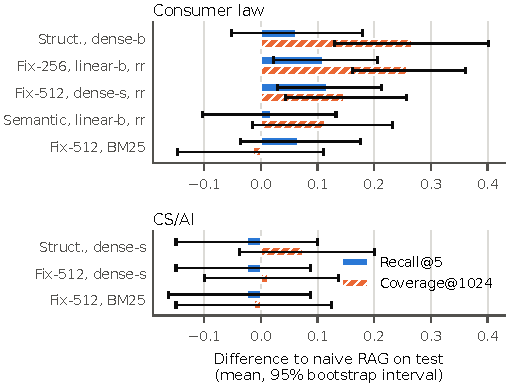
\includegraphics[width=\columnwidth]{figures/retrieval_deltas_ieee.pdf}
\caption{Retrieval on test: paired differences to naive RAG in Recall@5 and coverage at \V{gen.budget} tokens, with 95\% bootstrap intervals. Labels: chunker, retriever and encoder size (s/b); rr = reranking. Naive RAG reaches Recall@5 \V{cl.ret.naive.r5} and coverage \V{cl.ret.naive.cov1024} on consumer law (CS/AI: \V{cs.ret.naive.r5} and \V{cs.ret.naive.cov1024}); the other absolute values are in the extended version~\cite{shukla2026veridexext}.}
\label{fig:retrieval}
\end{figure}

On consumer law (Fig.~\ref{fig:retrieval}), the dev-selected configuration (structural chunks, dense bge-base) raises coverage at \V{gen.budget} tokens from \V{cl.ret.naive.cov1024} to \V{cl.ret.struct-b.cov1024} (\V{cl.ret.struct-b.dcov} \V{cl.ret.struct-b.dcovci}; Holm-adjusted $p=\V{prim.cl.cov.pholm}$; strict relevance: \V{cl.strict.strict.d} \V{cl.strict.strict.dci}), while its Recall@5 difference is \V{cl.ret.struct-b.dr5sig} (\V{cl.ret.struct-b.dr5} \V{cl.ret.struct-b.dr5ci}).
Both use the same encoder, so the difference comes from chunking: structural chunks, which carry their heading path, are short (mean \V{cl.tok.structural} tokens against \V{cl.tok.fixed512}), so a \V{gen.budget}-token budget holds more distinct provisions than the two fixed-512 windows it admits.
Coverage goes with correctness, although both depend on the question type: G2 answers \V{cl.cc.G2.all} of answerable consumer-law questions correctly when every gold provision is in its context and \V{cl.cc.G2.part} otherwise (\V{cl.cc.G2.all.n} and \V{cl.cc.G2.part.n} questions).
Short chunks alone may explain much of the gain: fixed-256 windows reach similar coverage (\V{cl.ret.f256-hyb-rr.dcov} \V{cl.ret.f256-hyb-rr.dcovci}), although that configuration also uses hybrid retrieval and reranking, which raise its latency to \V{cl.ret.f256-hyb-rr.lat}\,ms per query against \V{cl.ret.struct-b.lat}\,ms; we did not test section-aligned and fixed chunks of equal length.
On CS/AI, whose long sections the structural chunker splits more often (\V{cs.split.structural} against \V{cl.split.structural}), no difference is significant, including structural against fixed-512 chunks with the same encoder (coverage \V{cs.dret.struct-s-f512-s.dcov} \V{cs.dret.struct-s-f512-s.dcovci}; not shown in Fig.~\ref{fig:retrieval}).

% Generated by scripts/paper_tables.py -- do not edit by hand.
\begin{table*}[t]
\centering\footnotesize\setlength{\tabcolsep}{3.6pt}
\begin{tabular}{@{}llrrrrrrrrrrr@{}}
\toprule
Coll. & Sys. & Ans. & Faith. & Uncit. & Sup. & Corr. & Overall & Wrong & Refusal & F.\,abst. & Calls & p50 s \\ \midrule
Consumer law & G1 & 0.647 & 0.179 & 0.138 & 0.220 & 0.321 & 0.376 & 38 & 0.882 & 0.221 & 1.05 & 26.7 \\
 & G2 & 0.776 & 0.745 & 0.122 & 0.862 & 0.485 & 0.576 & 34 & 1.000 & 0.029 & 1.00 & 32.5 \\
 & G3 & 0.659 & 0.866 & 0.000 & 0.871 & 0.518 & 0.541 & 27 & 1.000 & 0.176 & 1.00 & 32.5 \\
 & G4 & 0.576 & 0.878 & 0.000 & 0.887 & 0.571 & 0.529 & 21 & 1.000 & 0.279 & 1.98 & 42.3 \\
 & G5 & 0.412 & 0.829 & 0.000 & 0.838 & 0.600 & 0.447 & 14 & 1.000 & 0.485 & 1.25 & 36.9 \\
 & G6 & 0.400 & 0.392 & 0.000 & 0.385 & 0.485 & 0.376 & 18 & 0.941 & 0.515 & 2.31 & 69.0 \\
 & G2H & 0.776 & 0.760 & 0.028 & 0.757 & 0.562 & 0.600 & 30 & 0.882 & 0.059 & 1.00 & 1.2 \\
\midrule
CS/AI & G1 & 0.536 & 0.011 & 0.622 & 0.059 & 0.400 & 0.500 & 18 & 1.000 & 0.250 & 1.00 & 31.6 \\
 & G2 & 0.571 & 0.312 & 0.447 & 0.462 & 0.406 & 0.518 & 19 & 1.000 & 0.200 & 1.00 & 31.1 \\
 & G3 & 0.393 & 0.455 & 0.000 & 0.500 & 0.409 & 0.446 & 13 & 1.000 & 0.450 & 1.00 & 31.1 \\
 & G4 & 0.321 & 0.444 & 0.000 & 0.444 & 0.444 & 0.429 & 10 & 1.000 & 0.550 & 1.77 & 39.5 \\
 & G2H & 0.643 & 0.343 & 0.089 & 0.366 & 0.556 & 0.643 & 16 & 1.000 & 0.100 & 1.00 & 0.6 \\
\bottomrule
\end{tabular}
\caption{Answer quality on the test split. G1 naive RAG (Fix-512, dense-b); G2 dev-best structural retrieval; G3 = G2 with the guards as a release filter (no revision); G4 = G2 + guards + critic, with one revision round; G5 = G4 + dev-tuned score threshold; G6 = Fix-256 hybrid with reranking, guards and critic; G2H = G2 with gpt-oss-120b (others: qwen2.5:3b). Ans.\ = share answered; Faith.\ = released-answer faithfulness (mean over answers); Uncit.\ = share of released sentences without a citation and Sup.\ = NLI support of cited sentences (both pooled over sentences, so they do not combine into Faith.); Corr.\ = correct among answered answerable questions (the accuracy of released answers); Wrong = released answers judged incorrect; F.\,abst.\ = false abstention; Calls = mean LLM calls per question (critic, revision and JSON-repair calls included); p50 s = median latency. Metrics: \S\ref{sec:setup}; citation precision and recall: Table~\ref{tab:genextra}.}
\label{tab:generation}
\end{table*}

% Generated by scripts/paper_tables.py -- do not edit by hand.
\begin{table}[t]
\TabCaption{tab:bootstrap}{Main paired differences on the test split with 95\% bootstrap intervals (\V{boot.n} resamples over questions)}{Released faithfulness = faithfulness over the answers each system releases (uncited sentences count as unsupported); support of cited sentences = NLI support among released sentences that carry a citation. Bold = interval excludes 0 (a bound at 0.000 counts as including 0); for overall accuracy, bold also requires a paired permutation test to give $p<0.05$ (uncorrected), and $^\dagger$ marks an interval that excludes 0 without it (few questions differ). -- = not computed. Faithfulness on jointly answered questions, correct refusal and further pairs: \ExtRef{Table}{tab:bootstrap-full}.}%
\centering\scriptsize\setlength{\tabcolsep}{2.2pt}
\begin{tabular}{@{}lrrr@{}}
\toprule
\makecell[l]{Comparison\\(what changes)} &\makecell[r]{$\Delta$ Released\\faithfulness} & \makecell[r]{$\Delta$ Support of\\cited sentences} & \makecell[r]{$\Delta$ Overall\\accuracy} \\ \midrule
\multicolumn{4}{@{}l}{\emph{Consumer law}} \\
\makecell[l]{G2$-$G1\\{retrieval}} & \makecell[r]{\textbf{+0.566}\\{\textbf{[0.420, 0.715]}}} & \makecell[r]{\textbf{+0.642}\\{\textbf{[0.491, 0.781]}}} & \makecell[r]{\textbf{+0.200}\\{\textbf{[0.094, 0.306]}}} \\[1pt]
\makecell[l]{G3$-$G2\\{guards}} & \makecell[r]{\textbf{+0.121}\\{\textbf{[0.048, 0.191]}}} & \makecell[r]{+0.009\\{[$-$0.012, 0.042]}} & \makecell[r]{$-$0.035\\{[$-$0.082, 0.000]}} \\[1pt]
\makecell[l]{G4$-$G2\\{guards + critic}} & \makecell[r]{\textbf{+0.133}\\{\textbf{[0.053, 0.214]}}} & \makecell[r]{+0.025\\{[$-$0.019, 0.081]}} & \makecell[r]{$-$0.047$^\dagger$\\{[$-$0.094, $-$0.012]}} \\[1pt]
\makecell[l]{G4$-$G3\\{critic + revision}} & \makecell[r]{+0.011\\{[$-$0.022, 0.054]}} & \makecell[r]{+0.016\\{[$-$0.021, 0.060]}} & \makecell[r]{$-$0.012\\{[$-$0.047, 0.024]}} \\[1pt]
\makecell[l]{G5$-$G4\\{threshold}} & \makecell[r]{\textbf{$-$0.049}\\{\textbf{[$-$0.106, $-$0.014]}}} & -- & \makecell[r]{\textbf{$-$0.082}\\{\textbf{[$-$0.153, $-$0.035]}}} \\[1pt]
\makecell[l]{G2H$-$G2\\{generator, budget}} & \makecell[r]{+0.015\\{[$-$0.121, 0.150]}} & \makecell[r]{$-$0.104\\{[$-$0.219, 0.007]}} & \makecell[r]{+0.024\\{[$-$0.071, 0.129]}} \\[1pt]
\midrule
\multicolumn{4}{@{}l}{\emph{CS/AI}} \\
\makecell[l]{G2$-$G1\\{retrieval}} & \makecell[r]{\textbf{+0.301}\\{\textbf{[0.156, 0.462]}}} & \makecell[r]{\textbf{+0.403}\\{\textbf{[0.184, 0.615]}}} & \makecell[r]{+0.018\\{[$-$0.089, 0.125]}} \\[1pt]
\makecell[l]{G3$-$G2\\{guards}} & \makecell[r]{\textbf{+0.142}\\{\textbf{[0.059, 0.263]}}} & \makecell[r]{+0.038\\{[0.000, 0.101]}} & \makecell[r]{$-$0.071$^\dagger$\\{[$-$0.143, $-$0.018]}} \\[1pt]
\makecell[l]{G4$-$G2\\{guards + critic}} & \makecell[r]{+0.132\\{[$-$0.023, 0.321]}} & \makecell[r]{$-$0.017\\{[$-$0.185, 0.167]}} & \makecell[r]{$-$0.089$^\dagger$\\{[$-$0.161, $-$0.018]}} \\[1pt]
\makecell[l]{G4$-$G3\\{critic + revision}} & \makecell[r]{$-$0.010\\{[$-$0.149, 0.140]}} & \makecell[r]{$-$0.056\\{[$-$0.220, 0.120]}} & \makecell[r]{$-$0.018\\{[$-$0.054, 0.000]}} \\[1pt]
\makecell[l]{G2H$-$G2\\{generator, budget}} & \makecell[r]{+0.030\\{[$-$0.172, 0.242]}} & \makecell[r]{$-$0.096\\{[$-$0.306, 0.153]}} & \makecell[r]{+0.125$^\dagger$\\{[0.018, 0.232]}} \\[1pt]
\bottomrule
\end{tabular}
\TabNotes
\end{table}

\ifshowprimary% Generated by scripts/paper_tables.py -- do not edit by hand.
\begin{table*}[t]
\TabCaption{tab:primary}{Primary comparisons with paired permutation tests (10,000 permutations) and Holm's correction across the 7 tests}{This family was fixed after the first draft, as a robustness check of the bootstrap intervals. Discord.\ = questions only the first system got right / only the second.}%
\centering\footnotesize\setlength{\tabcolsep}{5pt}
\begin{tabular}{@{}llrrrr@{}}
\toprule
Coll. & Comparison & $\Delta$ & $p$ & $p_{\mathrm{Holm}}$ & Discord. \\ \midrule
Cons.\ law & coverage@1024, structural $-$ naive & +0.267 & 0.0003 & 0.0021 & -- \\
CS/AI & coverage@1024, structural $-$ naive & +0.075 & 0.3364 & 0.6727 & -- \\
Cons.\ law & released faithfulness, G4 $-$ G2 & +0.133 & 0.0023 & 0.0138 & -- \\
Cons.\ law & overall accuracy, G4 $-$ G2 & $-$0.047 & 0.1214 & 0.3642 & 0/4 \\
Cons.\ law & overall accuracy, G2H $-$ G2 & +0.024 & 0.8136 & 0.8136 & 10/8 \\
CS/AI & released faithfulness, G4 $-$ G2 & +0.132 & 0.0830 & 0.3320 & -- \\
CS/AI & overall accuracy, G4 $-$ G2 & $-$0.089 & 0.0600 & 0.3000 & 0/5 \\
\bottomrule
\end{tabular}
\TabNotes
\end{table*}
\fi

\subsection{Generation and Faithfulness}
\label{sec:res-generation}

The retrieval change gives the largest gain on test (Tables~\ref{tab:generation} and~\ref{tab:bootstrap}): G2 improves on naive RAG in released-answer faithfulness and cited-sentence support on both collections, and in overall accuracy on consumer law only (\V{cl.boot.G2-G1.acc} \V{cl.boot.G2-G1.accci}).

Guards alone (G3) and guards with the critic (G4) raise released-answer faithfulness over G2 on consumer law (\V{cl.rel.G3-G2} \V{cl.rel.G3-G2ci}; \V{cl.rel.G4-G2} \V{cl.rel.G4-G2ci}, Holm-adjusted $p=\V{prim.cl.G4-G2.rel.pholm}$), but the metric counts uncited sentences as unsupported and the citation guard withholds exactly the answers that contain them (\V{cl.sent.G2.uncited} of G2's released sentences on consumer law, \V{cs.sent.G2.uncited} on CS/AI).
Among cited sentences, NLI support does not change significantly on either collection (consumer law: \V{cl.cit.G4-G2} \V{cl.cit.G4-G2ci}), and the critic with its revision round adds nothing measurable over the guard filter (G4$-$G3: \V{cl.rel.G4-G3} \V{cl.rel.G4-G3ci}) while nearly doubling the LLM calls.
The verifier therefore mainly enforces the citation format and shows no measurable ability to detect cited but unsupported content, in line with weak self-critique by small models~\cite{huang2024selfcorrect}.
Filtering does reduce wrong answers: on consumer law G4 releases \V{cl.sent.G4.wrong} answers judged incorrect against \V{cl.sent.G2.wrong} for G2, at the price of \V{cl.sent.G4.correct} correct answers against \V{cl.sent.G2.correct}.
The overall-accuracy differences of G4 to G2 rest on \V{prim.cl.G4-G2.acc.loss} (consumer law) and \V{prim.cs.G4-G2.acc.loss} (CS/AI) questions that G2 got right and G4 did not, with none in the other direction; the permutation tests give $p=\V{prim.cl.G4-G2.acc.p}$ and $p=\V{prim.cs.G4-G2.acc.p}$, not significant even before correction.
G2 and G4 refuse every unanswerable question, but these are easy; naive RAG already refuses \V{cl.gen.G1.refusaln} of \V{cl.gen.nunans} and \V{cs.gen.G1.refusaln} of \V{cs.gen.nunans}.
G6, built on the configuration with the best dev Recall@5, is far worse than G4 (released-answer faithfulness \V{cl.rel.G6-G4} \V{cl.rel.G6-G4ci}).

A larger generator helps, if at all, on the textbooks.
G2H replaces qwen2.5:3b by \gptoss{}, which also brings a larger context budget, a larger output limit and hidden reasoning. On consumer law its differences to G2 have wide intervals (Table~\ref{tab:bootstrap}), so the data neither detect a difference nor show that there is none.
On CS/AI it raises accuracy by \V{cs.boot.G2H-G2.acc} \V{cs.boot.G2H-G2.accci}: it abstains less on answerable questions (\V{cs.gen.G2H.falseabspct} against \V{cs.gen.G2.falseabspct}) and more of its answers are correct. The gain rests on \V{sec.cs.G2H-G2.acc.win} questions only G2H got right against \V{sec.cs.G2H-G2.acc.loss} only G2 got right, and a paired permutation test, outside the corrected family, gives $p=\V{sec.cs.G2H-G2.acc.p}$; released-answer faithfulness does not change significantly.
On consumer law G2H cites several passages in one sentence more often (\V{cl.sent.G2H.multi} of \V{cl.sent.G2H.n} sentences against \V{cl.sent.G2.multi} of \V{cl.sent.G2.n}), which a single-passage judge cannot credit; its cited-sentence support changes by \V{cl.cit.G2H-G2} \V{cl.cit.G2H-G2ci}.
Run on the provider's hardware, it is much faster than the local model on the laptop CPU (median \V{cl.gen.G2H.p50}\,s against \V{cl.gen.G2.p50}\,s on consumer law).

\ifshowdomain
On the textbooks, faithfulness is lower at every stage (G2: \V{cs.gen.G2.faith} against \V{cl.gen.G2.faith}), largely because the small model leaves \V{cs.sent.G2.uncited} of its CS/AI sentences uncited; G4 then withholds \V{cs.gen.G4.falseabspct} of the answerable CS/AI questions (the guard filter alone, G3: \V{cs.gen.G3.falseabspct}).
\fi

\subsection{Abstention}
\label{sec:res-abstention}

\ifshowselective
\begin{figure}[t]
\centering
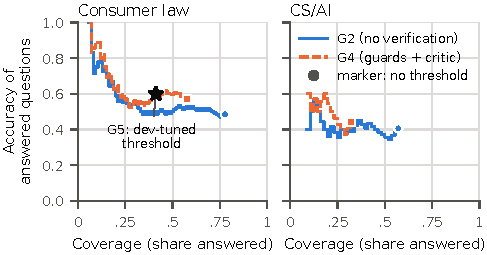
\includegraphics[width=\columnwidth]{figures/selective.pdf}
\caption{Accuracy of released answers against coverage (share of questions answered) when G2 and G4 also abstain below a top-1 retrieval-score threshold swept over the test scores (descriptive; points with at least five answered questions). Circle (G2) and square (G4) at the right end: no threshold. Star: G5, i.e.\ G4 with the threshold tuned on dev.}
\label{fig:selective}
\end{figure}
\fi

G5 abstains before any LLM call when the top-1 dense cosine falls below a threshold (\V{abs.thr}) tuned on dev for the abstention F1 of the threshold alone, although G4 already refuses every unanswerable question.
On test it abstained before generation on \V{cl.gen.G5.lowretrievalscore} questions, raised false abstention from \V{cl.gen.G4.falseabspct} to \V{cl.gen.G5.falseabspct}, lowered released-answer faithfulness by \V{cl.rel.G5-G4} \V{cl.rel.G5-G4ci} and changed accuracy relative to G4 by \V{cl.boot.G5-G4.acc} \V{cl.boot.G5-G4.accci} (all \V{sec.cl.G5-G4.acc.loss} discordant questions favor G4; permutation $p=\V{sec.cl.G5-G4.acc.p}$).
Besides the small dev set, the tuning objective explains this: the score separates answerable from unanswerable test questions well (area under the ROC curve \V{cl.ret.struct-b.auroc}), but G4 left no unanswerable questions for it to catch.
\ifshowselective In the descriptive sweep of Fig.~\ref{fig:selective}, at\else In a descriptive sweep of the threshold, at\fi{} G4's answer rate (\V{cl.sel.G4.cov0}), G2 with a score threshold reaches an accuracy of released answers of \V{cl.sel.G2.atG4}, against \V{cl.sel.G4.acc0} for G4; abstaining at random would keep G2's \V{cl.sel.G2.acc0}. The verifier thus selects somewhat better than a retrieval-score rule at an equal answer rate, a descriptive comparison we did not test.

\ifshowerrors% Generated by scripts/paper_tables.py -- do not edit by hand.
\begin{table}[t]
\centering\footnotesize\setlength{\tabcolsep}{4pt}
\begin{tabular}{@{}lrrr@{}}
\toprule
Category & Cons.\ law & CS/AI & Total \\ \midrule
Retrieval miss & 2 & 3 & 5 \\
Chunk boundary & 0 & 0 & 0 \\
Synthesis error & 4 & 0 & 4 \\
Verifier false reject & 0 & 4 & 4 \\
Verifier false accept & 0 & 0 & 0 \\
Evaluation artefact & 5 & 2 & 7 \\
\midrule
Sampled failures & 11 & 9 & 20 \\
\bottomrule
\end{tabular}
\caption{Error categories of 20 G4 test failures (of \V{cl.err.nfail} consumer-law and \V{cs.err.nfail} CS/AI failures), sampled with seed \V{err.seed} in proportion to the failures per collection.}
\label{tab:errors}
\end{table}
\fi

\subsection{Error Analysis}
\label{sec:res-errors}

We sampled \V{err.n} G4 test failures (an answerable question answered incorrectly or withheld, or an unanswerable one answered), \V{cl.err.nsample} on consumer law and \V{cs.err.nsample} on CS/AI in proportion to their failures.
Rule-based pre-labels were checked against each record, and the final labels were assigned with AI assistance (\V{err.agree} of \V{err.n} pre-labels kept).
The largest group\ifshowerrors{} in Table~\ref{tab:errors}\fi, \emph{evaluation artifacts} (\V{err.evalartifact}), are not system errors: correct answers that the NLI judge does not entail (code, a formula, a short noun phrase), one gold answer that contradicts its source and one ambiguous question.
\emph{Retrieval misses} (\V{err.retrievalmiss}) ranked the gold provision below what fit in the context; in \emph{synthesis errors} (\V{err.synthesiserror}) the evidence was in the context but the answer was wrong or did not answer.
All \emph{verifier false rejects} (\V{err.verifierfalsereject}) are on CS/AI: correct answers withheld, three because a sentence lacked its citation tag and one after a critic revision request.
